% Status update 1 (10 November 2023), ported from Pages.
% Compile with LuaLaTeX: latexmk -lualatex statusupdate_1.tex
\documentclass[12pt]{article}

\usepackage[a4paper, left=25mm, right=25mm, top=30mm, bottom=25mm, footskip=12mm]{geometry}
\usepackage[ngerman]{babel}
\usepackage{fontspec}
\usepackage{xcolor}
\usepackage{enumitem}
\usepackage{titlesec}
\usepackage{graphicx}
\usepackage{fancyhdr}
\usepackage{tikz}
\usetikzlibrary{arrows.meta}

\setmainfont{TeX Gyre Heros}
\linespread{1.1}
\AtBeginDocument{\raggedright}
\hyphenpenalty=10000
\setlength{\parindent}{0pt}
\setlength{\parskip}{0pt}
\definecolor{titlegray}{gray}{0.35}
\definecolor{rulegray}{gray}{0.45}

% Page number bottom left
\pagestyle{fancy}
\fancyhf{}
\fancyfoot[L]{\thepage}
\renewcommand{\headrulewidth}{0pt}

% Sections: thin rule above, regular weight
\titleformat{\section}[block]{{\color{rulegray}\titlerule[0.4pt]}\vspace{4pt}\normalfont\large}{}{0pt}{}
\titlespacing*{\section}{0pt}{14pt}{6pt}

% Dash bullets and numbered steps
\setlist[itemize]{label=-, leftmargin=12pt, labelsep=6pt, itemsep=6pt, topsep=0pt}
\setlist[enumerate]{leftmargin=36pt, itemsep=4pt, topsep=6pt, label=\arabic*.}

\begin{document}

Friday, 10. November 2023\\
Leonhard Driesch

\vspace{8pt}
{\color{titlegray}\bfseries\fontsize{20}{25}\selectfont Update zur Automatic Colony Counting\\Bachelorarbeit\par}
\vspace{8pt}

\section{Treffen mit Prof. Jiang}
\begin{itemize}
  \item Ich habe mich mit Professor Jiang zusammengesetzt und die ersten Bilder begutachtet die Sebastian mir zukommen lassen hat
  \item Wir haben festgestellt, dass die Form der Bakterienkolonien meist rund ist und sich vom Hintergrund stark absetzt
  \item Prof. Jiang hat mir empfohlen, mich zunächst an einer simplen Computer Vision Pipeline mit bekannten Algorithmen zu versuchen
\end{itemize}

\section{Computer Vision Pipeline}
\begin{itemize}
  \item Mithilfe von OpenCV habe ich in einem Jupyter Notebook angefangen herumzuexperimentieren und habe dabei folgende Pipeline entworfen (Beispielbilder weiter unten zu finden):
  \begin{enumerate}
    \item Bild in Graustufen umwandeln
    \item Leichten Gaussian Blur anwenden um kleine Unreinheiten auf dem Bild zu eliminieren
    \item Petri Schale ausschneiden (Hintergrund entfernen)
    \item Mit einem Hough Circles Transform Bakterienkolonien markieren und zählen
  \end{enumerate}
  \item Ich habe die Hyperparameter mit einem Grid-Search ein wenig optimiert, und habe somit folgende Ergebnisse erreicht (Vergleich handgezählt vs.\ computergezählt):

  \vspace{6pt}
  \hspace*{22pt}Median relativer Fehler: 8\%, durchschnittlich 20\%

  \vspace{6pt}
  \hspace*{22pt}Median absoluter Fehler: 0, durchschnittlich werden 98 zu wenig gezählt
  \item Der Ansatz funktioniert also gut für “normale” Bilder, also ca. zwischen 1 und 150 Kolonien
  \item Der Ansatz funktioniert sehr schlecht für Bilder mit äußerst vielen Kolonien (1000+)
\end{itemize}

\newpage
\vspace*{-14pt}
\section{Interface}
\begin{itemize}
  \item Ich habe mir erste Gedanken über ein User Interface gemacht. Es ist wichtig, dass man als Nutzer des Programmes nachvollziehen kann, welche Kolonien erkannt wurden und ggf. das Ergebnis korrigieren kann, da keine 100\%ig zuverlässige Erkennung möglich ist
  \item Habe hier aber ein paar Ansätze, kann aber noch nichts Spektakuläres zeigen
\end{itemize}

\section{Weiteres Vorgehen}
\begin{itemize}
  \item Bisher wurde ja noch kein Machine Learning verwendet, die Idee wäre jetzt, mithilfe der algorithmischen Methode Trainingsdaten zu erstellen und darauf bspw.\ ein Image Segmentation Modell zu trainieren
  \item Zum genauen Vorgehen werde ich mir nochmal den Rat von Prof. Jiang einholen
  \item Ich bin erstmal bis zum 22. November verhindert, kann mich aber anschließend Vollzeit auf die Bachelorarbeit fokussieren.
\end{itemize}

\vspace{40mm}
Hier unten folgen noch die Beispielbilder
\begin{tikzpicture}[overlay]
  \draw[line width=1.2pt, -{Latex[length=9pt, width=7pt]}] (3mm, 10mm) -- (7mm, -87mm);
\end{tikzpicture}

\newgeometry{left=12mm, right=12mm, top=8mm, bottom=25mm, footskip=12mm}
\begin{center}
  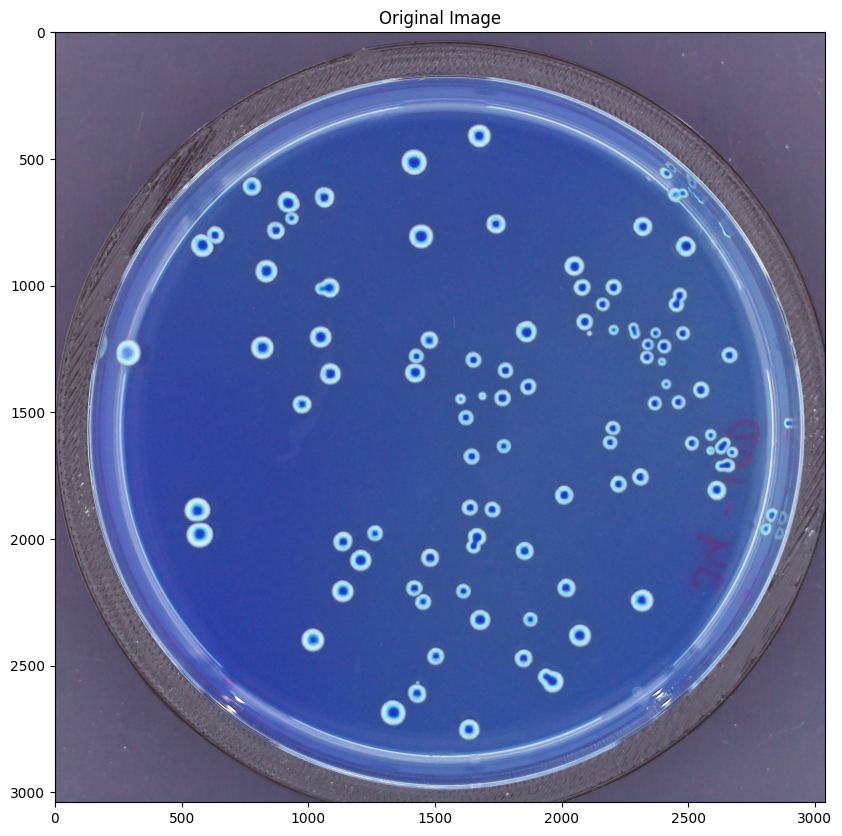
\includegraphics[width=84mm]{images/step1.png}\hspace{5mm}%
  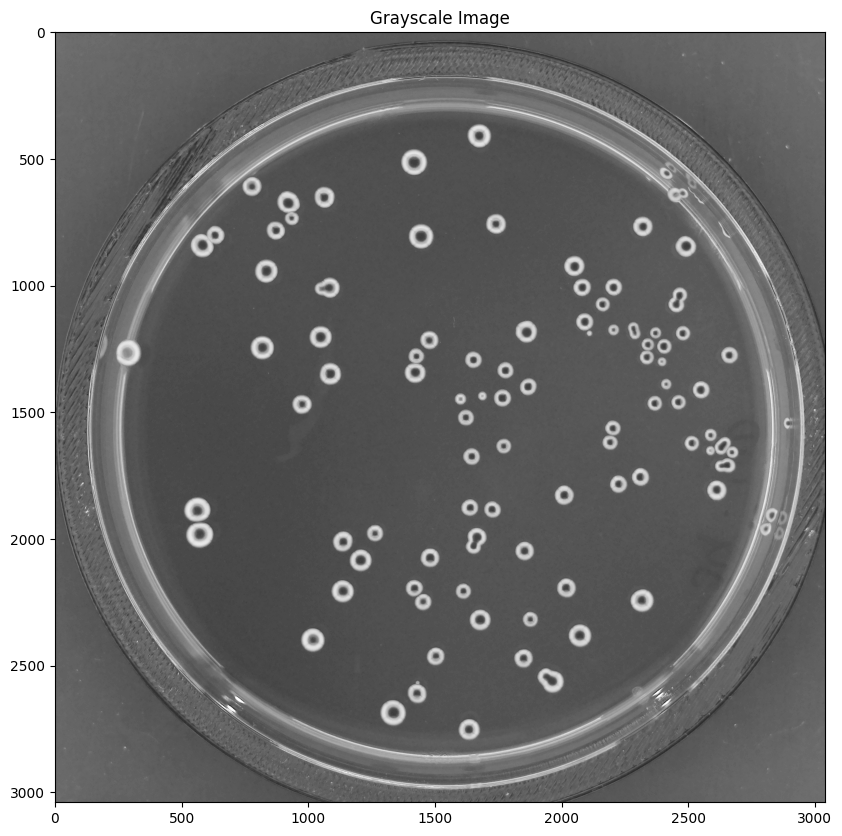
\includegraphics[width=84mm]{images/step2.png}\\[1mm]
  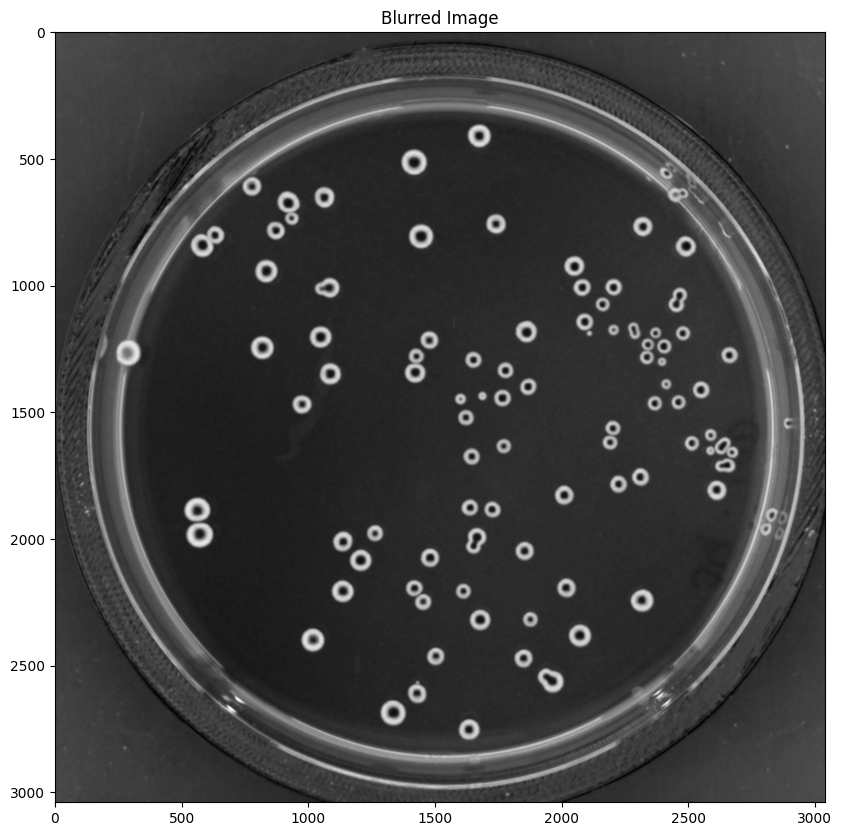
\includegraphics[width=84mm]{images/step3.png}\hspace{5mm}%
  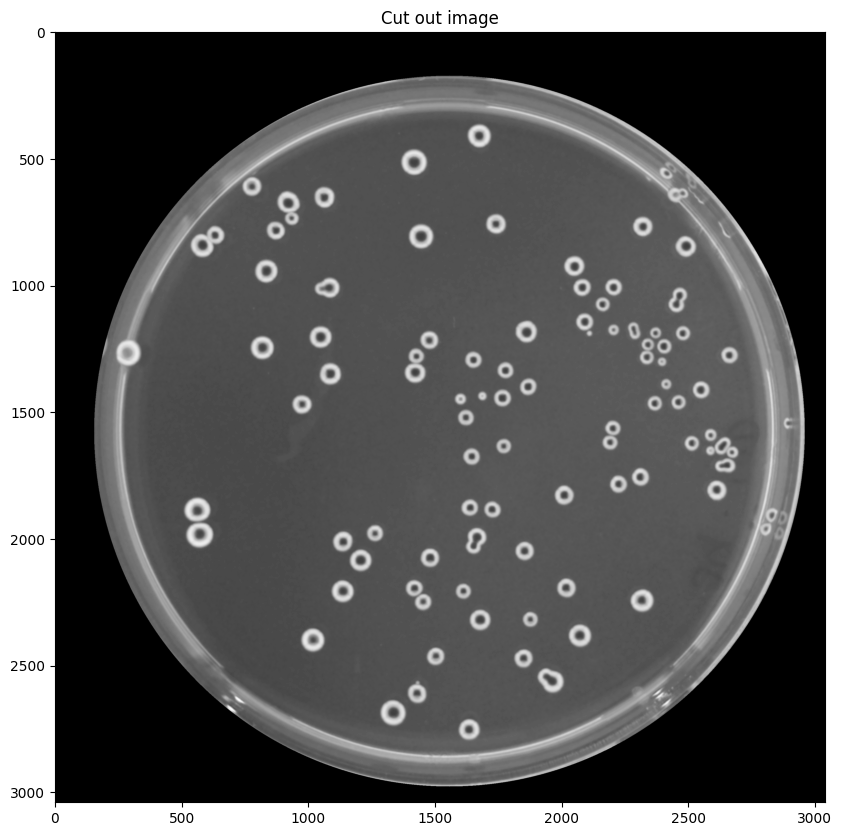
\includegraphics[width=84mm]{images/step4.png}\\[1mm]
  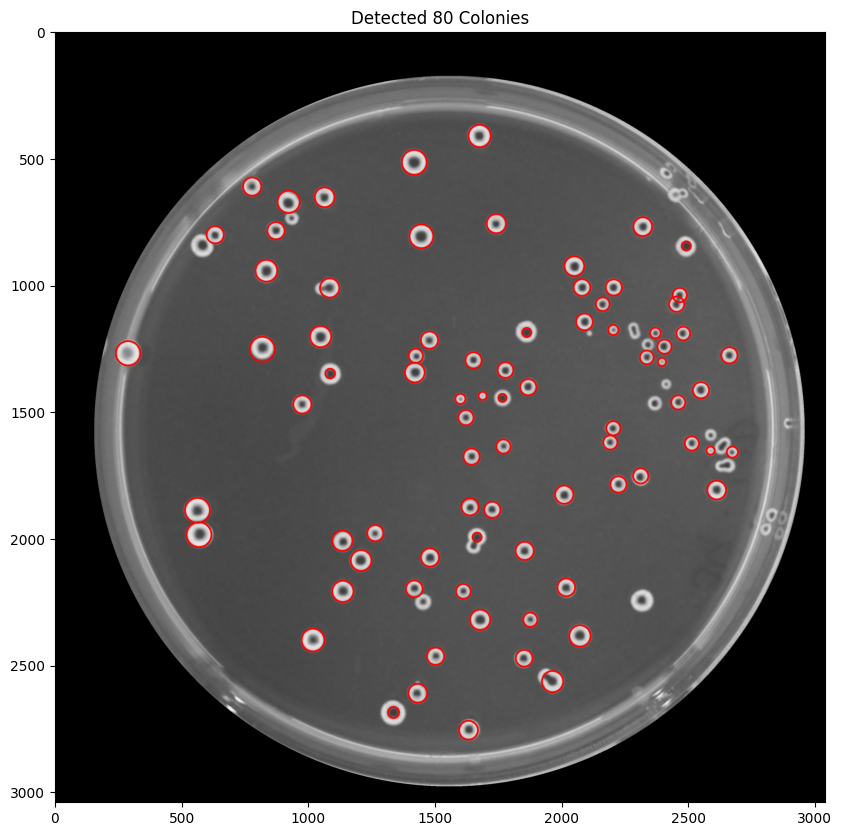
\includegraphics[width=84mm]{images/step5.png}\hspace{5mm}%
  \hspace*{84mm}
\end{center}

\end{document}
